\subsection{同一个动量可以对应相反的最优方向}
固定$M=\operatorname{diag}(1,0.08)$时，NS1和NS5的方向比例分别为0.387和1.372，
幅度匹配后的极因子误差分别为0.413和0.155。
图\ref{fig:v2geometry}(a)在每个位置为两个方向分别求最优标量步长，
以$J_5/J_1$呈现方向本身的收益差异。取$\rho=0.1$时，分界$\kappa_*=0.117$。
当弱梯度方向的曲率高于该分界，NS1在这一方向分配的更新更小，获得更高的下降收益。
二维相图的5120个网格点均符合命题\ref{prop:v2boundary}的排序预测。

\begin{figure}[htbp]\centering
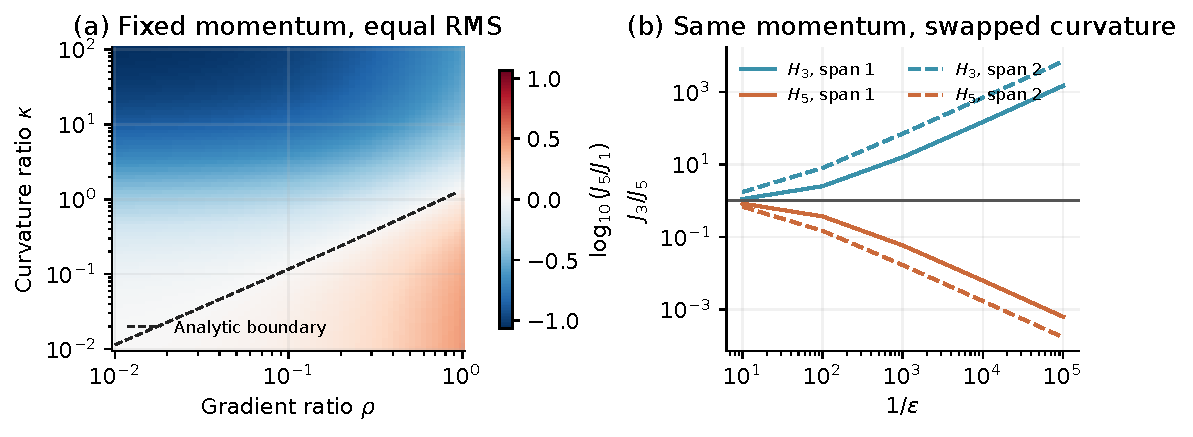
\includegraphics[width=\linewidth]{figures_v2/v2_geometry.pdf}
\caption{更新方向的收益分界。(a) 固定动量，改变梯度比$\rho$和曲率比$\kappa$。虚线为解析分界。
(b) 固定梯度与动量，分别沿NS3和NS5构造低曲率方向，绘出10个种子的几何平均收益比。}
\label{fig:v2geometry}
\end{figure}

在$16\times16$矩阵的曲率置换中，两个目标的Hessian特征值、初始梯度和候选谱误差逐项相同。
取$\epsilon=10^{-5}$，三个正谱跨度的30对目标全部反转NS3与NS5的排序。
将低曲率方向设置为NS3时，$J_3/J_5$的中位数为1947。置换为NS5时，$J_5/J_3$的中位数为1985。
该受控构造把收益差定位到方向与曲率的相对关系，差距随$1/\epsilon$增长，
与定理\ref{thm:v2reversal}的收益比一致。

\subsection{谱近似误差与优化收益采用不同的排序}
在更广泛的矩阵实验中，三种经验NS深度的更新幅度相同。
表\ref{tab:v2matrix}按梯度奇异值的对数跨度统计，极因子误差最小的候选在834个状态中的收益低于最优候选，
总计990个具有可区分收益的状态。
平坦谱、零噪声时三个方向重合，90个状态的收益并列。
图\ref{fig:v2errorgain}进一步比较固定条件数100下的两种曲率排列。
高曲率沿梯度主方向排列时，较平坦的更新谱可以减小曲率代价。
高曲率集中在尾部时，将更多更新能量分配给尾部会增加二阶代价。

\begin{table}[htbp]\centering
\caption{幅度匹配NS的谱误差和线优化收益。每个谱跨度含270个位置，来自10个配对种子。}
\label{tab:v2matrix}
\begin{tabular}{rrrr}
\toprule
对数谱跨度 & 非并列状态 & 误差最小候选收益次优 & 收益并列 \\ \midrule
0 & 180 & 97 & 90 \\
0.5 & 270 & 236 & 0 \\
1 & 270 & 237 & 0 \\
2 & 270 & 264 & 0 \\
\bottomrule
\end{tabular}

\end{table}

\begin{figure}[htbp]\centering
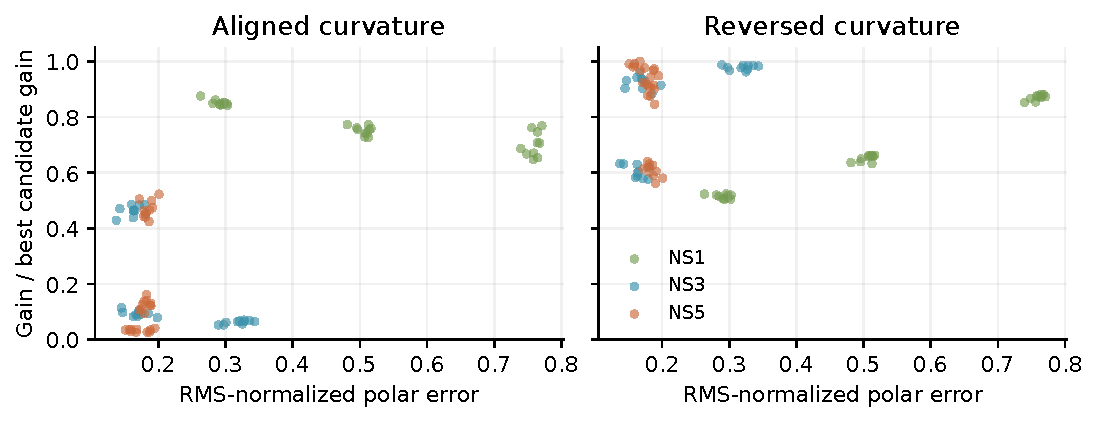
\includegraphics[width=\linewidth]{figures_v2/v2_error_gain.pdf}
\caption{条件数100、无噪声下的极因子误差与相对收益。正谱跨度及种子各自形成一个位置。
左图的低曲率沿梯度主方向排列，右图把高曲率移到梯度主方向。}
\label{fig:v2errorgain}
\end{figure}

分别选择学习率后，500步轨迹仍显示深度与噪声的交互。
在条件数100、倒置曲率的轨迹中，无噪声时NS3的终点目标均值为$7.20\times10^{-10}$，
低于NS5的$5.71\times10^{-9}$。
加入相当于初始梯度范数10\%的噪声后，幅度匹配动量的终点为$3.10\times10^{-4}$，
NS3和NS5则分别为$8.44\times10^{-4}$和$8.41\times10^{-4}$。
靠近最优点时真实梯度总体减小，固定尺度的噪声在观测梯度中占据更高比例。
谱变换改变观测谱中各方向的相对更新量，因而深度的作用随噪声条件变化。
完整轨迹与种子间变动见附录图\ref{fig:v2trajectory}。

\subsection{在冻结模型上测量方向曲率}
对同一个锚点，每个候选都从相同权重出发。比较任意两个候选$i,j$时，
用$\widehat\Delta_i-\widehat\Delta_j$预测它们的收益顺序。
给定共同的步长倍率$s$，一阶差为$s(a_i-a_j)$，二阶差再减去$s^2(b_i-b_j)/2$。
因此只改变步长倍率也可能改变排序。批次$B$与$C$分别提供预测和实测，
由此区分二阶式对当前目标的拟合与排序在数据上的迁移。
以三个经验深度为候选，预测器的成对一致率等于预测顺序与实测顺序一致的比例。
另设选择损失，定义为批次$C$上的最大候选下降量减去所选候选的下降量。
每个锚点内部完成所有候选配对，再以训练种子为单位聚合。

以主实验固定NS5、种子0的第250次更新为例，NS1与NS5的一阶下降预测分别为0.0652和0.0138。
NS1的二阶代价为0.1813，NS5为0.0077。将两个候选施加到独立批次$C$后，
NS1的损失上升0.1306，NS5的损失下降0.0037。
在这一位置，NS1沿梯度取得较大的一阶进展，但其方向上的曲率消耗了这份收益。

36个锚点共有72组独立批次测量。实际步长下，216个候选对在同一批次上的收益差平均绝对误差，
由一阶预测的0.08310降至二阶预测的0.00690 nats/token。
图\ref{fig:v2calibration}显示了这一改进。高曲率方向上的一阶预测明显偏高，二阶项校正了这部分差距。

\begin{figure}[htbp]\centering
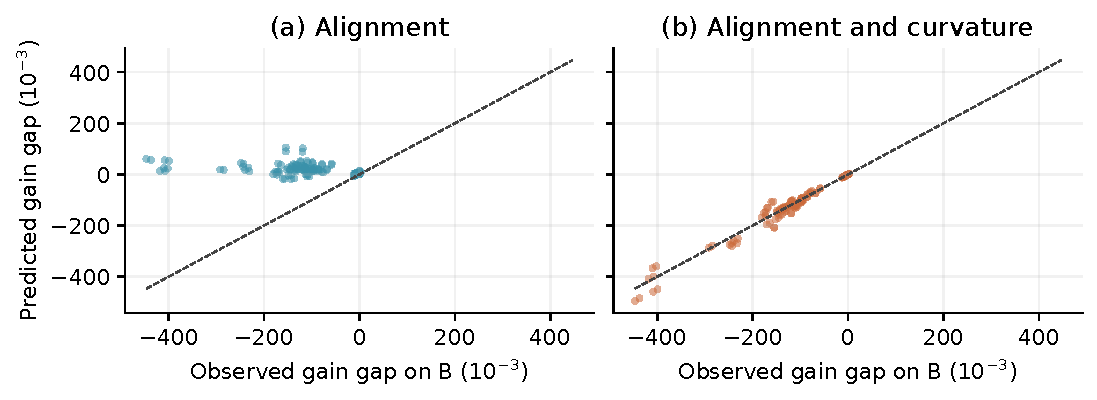
\includegraphics[width=\linewidth]{figures_v2/v2_curvature_calibration.pdf}
\caption{批次$B$上任意两个经验NS候选的下降量差。横轴为实际差值，纵轴为预测差值。虚线为两者相等。}
\label{fig:v2calibration}
\end{figure}

在独立批次$C$上，实际步长下的一阶排序一致率为25.0\%，二阶为94.4\%，谱误差为96.3\%。
以NS3与NS5为例，依据批次$B$的梯度对齐，NS3在72组比较中的57组占优。
计入方向曲率后，二阶式在8组中把NS3排在NS5前。独立批次$C$中实际也有8组NS3占优。
NS3较高的一阶收益经常伴随着较大的二阶代价。

当完整步长取实际步长的0.5、1和2倍时，NS5在72组比较中分别赢得45、64和72组。
半步长下谱误差的排序一致率降至85.6\%，二阶预测为83.8\%。
从半步长增至两倍步长时，NS3与NS5有27组排序反转。
二阶式预测了其中13组，并在另外18组给出反转预测。
图\ref{fig:v2ranking}同时给出排序一致率和选错深度造成的损失差。

\begin{figure}[htbp]\centering
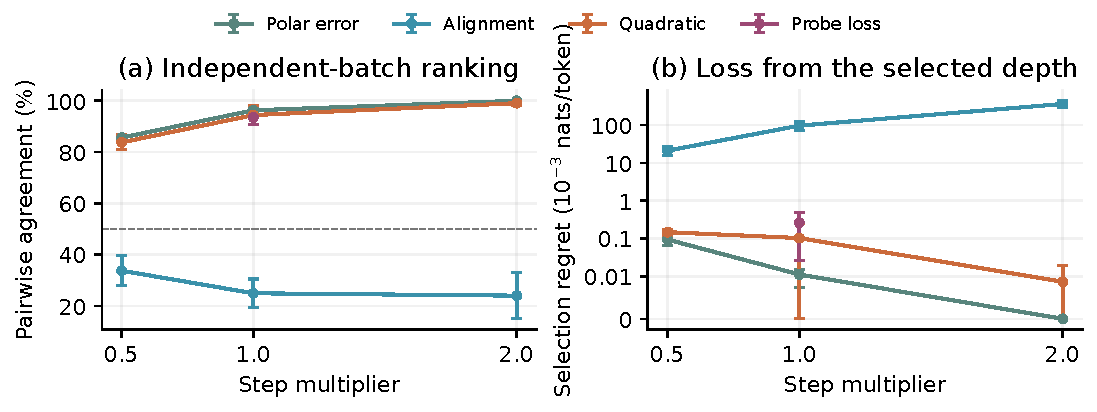
\includegraphics[width=\linewidth]{figures_v2/v2_probe_ranking.pdf}
\caption{独立批次上各选择依据的排序一致率与选择损失。误差条为训练种子间的一个样本标准差。
右图在零附近使用线性刻度，其余使用对数刻度。}
\label{fig:v2ranking}
\end{figure}

精确极因子也沿共同RMS生成完整步长。
在实际步长下，NS5与精确极因子的平均损失下降分别为$5.73\times10^{-4}$和$3.57\times10^{-4}$ nats/token。
72个配对测量中，NS5下降更多的有50个，精确极因子下降更多的有21个，另外1个在$10^{-7}$内并列。
在WikiText103冻结状态中，四类隐藏矩阵的归一化稳定秩随深度上升。
从NS1到NS5，小模型的平均值由0.018增至0.564，大模型由0.013增至0.569。
在相同总能量下，较深的候选把更新能量分配到更多奇异方向，见附录图\ref{fig:v2spectra}。

\subsection{固定深度在匹配训练中的收益}
在WikiText103的26.5M参数模型上，NS1、NS3和NS5使用相同的矩阵峰值学习率0.003，
每个隐藏矩阵的非衰减更新均具有相同的RMS。
三组的终点验证损失依次为5.5799、4.8954和4.8118 nats/token。
NS5相对NS3将终点验证损失平均降低0.0836，将测试损失平均降低0.0847。
三个配对种子上的两种损失均保持这一排序。
在这一配置中，增加深度改善了训练，同状态探测表明较浅方向经常承担更高的二阶代价。

AdamW经过相同规则的学习率筛选，终点验证损失为5.1240。
幅度匹配动量在独立选定的峰值学习率下取得5.3293。
表\ref{tab:v2main}列出各方法的学习率、终点验证损失和验证所选检查点的测试损失。
NS深度效应来自共同步长与共同辅助参数的配对对照。

\begin{table}[htbp]\centering\small
\caption{WikiText103的26.5M参数模型。每种方法使用三个配对种子，表中为均值和一个样本标准差。损失单位为nats/token。}
\label{tab:v2main}
\begin{tabular}{lrrr}
\toprule
方法 & 矩阵峰值学习率 & 终点验证损失 & 测试损失 \\ \midrule
AdamW & 0.0010 & $5.1240\pm0.0118$ & $5.1304\pm0.0118$ \\
Momentum & 0.0001 & $5.3293\pm0.0054$ & $5.3208\pm0.0079$ \\
NS1 & 0.0030 & $5.5799\pm0.0257$ & $5.5741\pm0.0251$ \\
NS3 & 0.0030 & $4.8954\pm0.0042$ & $4.9058\pm0.0025$ \\
NS5 & 0.0030 & $4.8118\pm0.0045$ & $4.8211\pm0.0079$ \\
Probe-NS & 0.0030 & $4.8150\pm0.0021$ & $4.8250\pm0.0064$ \\
Stage replay & 0.0030 & $4.8150\pm0.0021$ & $4.8250\pm0.0064$ \\
Error-NS & 0.0030 & $4.8118\pm0.0045$ & $4.8211\pm0.0079$ \\
RMS-Adam & 0.0010 & $5.1398\pm0.0053$ & $5.1456\pm0.0048$ \\
Canonical NS5 & 0.0030 & $4.8007\pm0.0064$ & $4.8106\pm0.0093$ \\
\bottomrule
\end{tabular}

\end{table}

\subsection{谱误差与目标反馈在常用深度上汇合}
Error-NS在主对照的30次选择中都选了NS5。Probe-NS选了28次NS5和2次NS3，
终点验证损失为4.8150，固定NS5为4.8118。
两个策略在训练中频繁遇到相同的最佳候选，这与冻结模型在实际步长下的排序结果一致。

三条阶段匹配重放与对应的反馈序列逐项相同。
种子0一直使用NS5。种子1和2在第900步改用NS3，在最终一步切回NS5。
最后一段中两种深度的驻留长度分别为100步和1步，保持实际更新频率便保留了它们的位置。
附录表\ref{tab:v2replay}给出每条序列和实际改动步数。

\input{v2_schedule_outcome}

\subsection{扩大规模、延长训练与改变更新尺度}
在51.1M参数模型中，隐藏矩阵参数增至25.17M。
固定NS5将WikiText103的终点验证损失从匹配AdamW的5.0354降至4.6493，
Probe-NS取得4.6506。该规模下的30次反馈选择有26次落在NS5。

在小模型的幅度消融中，固定AdamW学习率后，RMS-Adam取得5.1398，
标准AdamW为5.1240。固定NS5学习率后，Moonlight更新尺度取得4.8007，
逐矩阵匹配RMS为4.8118。两组消融直接测量了幅度变换对各自更新规则的影响。

\input{v2_transfer_outcome}

\begin{table}[htbp]\centering\small
\caption{模型规模、语料和训练长度的对照。各方法使用三个配对种子，损失单位为nats/token。}
\label{tab:v2transfer}
\input{v2_table_transfer}
\end{table}

\begin{figure}[htbp]\centering
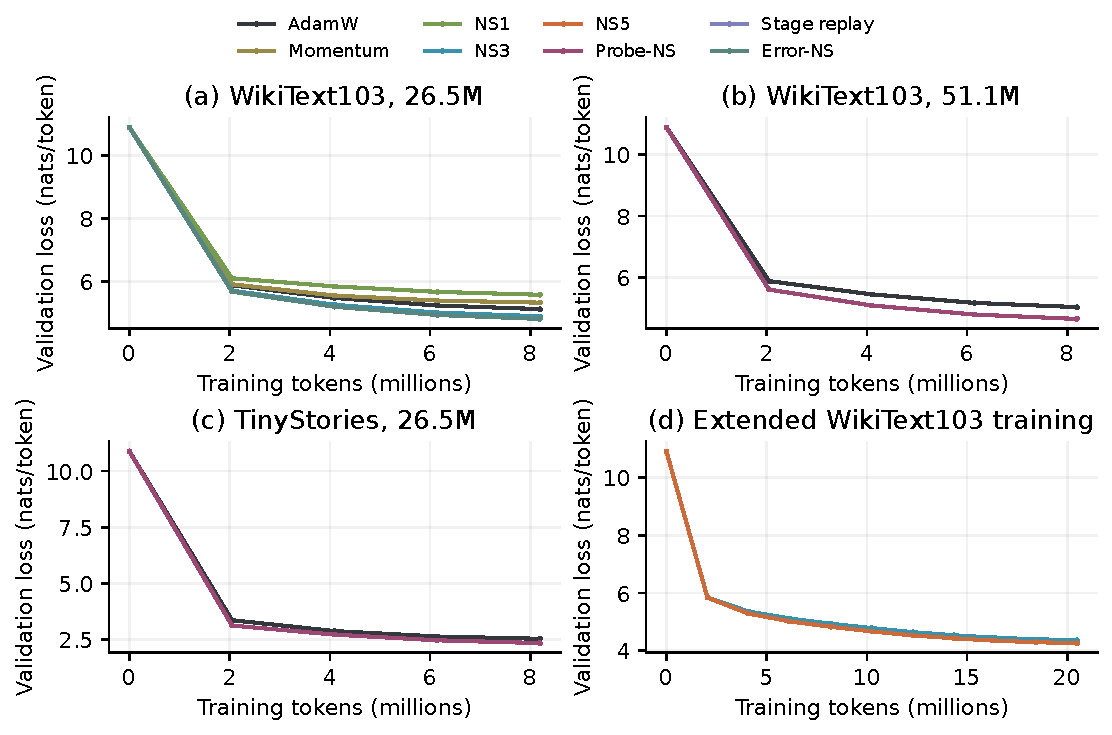
\includegraphics[width=\linewidth]{figures_v2/v2_training.pdf}
\caption{完整语言训练中的验证损失。各点为三个种子的均值，阴影为一个样本标准差。}
\label{fig:v2train}
\end{figure}

\input{v2_profile_outcome}



